\documentclass[a4paper]{article} 
\usepackage[francais]{babel}
\usepackage[utf8]{inputenc} % Required for including letters with accents
\usepackage[T1]{fontenc} % Use 8-bit encoding that has 256 glyphs

\usepackage{amsthm}
\usepackage{amsmath}
\usepackage{amssymb}
\usepackage{mathrsfs}
\usepackage{graphicx}
\usepackage{geometry}
\usepackage{stmaryrd}
\usepackage{tikz}
\usepackage{wrapfig}
\def \de {{\rm d}}
\usepackage{hyperref}
\hypersetup{
    colorlinks=true,
    linkcolor=blue,
    filecolor=magenta,      
    urlcolor=cyan,
}
 
\urlstyle{same}
\usepackage{tikz}


\usepackage{listings}
 \def \de {{\rm d}}
\definecolor{darkWhite}{rgb}{0.94,0.94,0.94}
 
\lstset{
  aboveskip=3mm,
  belowskip=-2mm,
  backgroundcolor=\color{darkWhite},
  basicstyle=\footnotesize,
  breakatwhitespace=false,
  breaklines=true,
  captionpos=b,
  commentstyle=\color{red},
  deletekeywords={...},
  escapeinside={\%*}{*)},
  extendedchars=true,
  framexleftmargin=16pt,
  framextopmargin=3pt,
  framexbottommargin=6pt,
  frame=tb,
  keepspaces=true,
  keywordstyle=\color{blue},
  language=python,
  literate=
  {²}{{\textsuperscript{2}}}1
  {⁴}{{\textsuperscript{4}}}1
  {⁶}{{\textsuperscript{6}}}1
  {⁸}{{\textsuperscript{8}}}1
  {€}{{\euro{}}}1
  {é}{{\'e}}1
  {è}{{\`{e}}}1
  {ê}{{\^{e}}}1
  {ë}{{\¨{e}}}1
  {É}{{\'{E}}}1
  {Ê}{{\^{E}}}1
  {û}{{\^{u}}}1
  {ù}{{\`{u}}}1
  {â}{{\^{a}}}1
  {à}{{\`{a}}}1
  {á}{{\'{a}}}1
  {ã}{{\~{a}}}1
  {Á}{{\'{A}}}1
  {Â}{{\^{A}}}1
  {Ã}{{\~{A}}}1
  {ç}{{\c{c}}}1
  {Ç}{{\c{C}}}1
  {õ}{{\~{o}}}1
  {ó}{{\'{o}}}1
  {ô}{{\^{o}}}1
  {Õ}{{\~{O}}}1
  {Ó}{{\'{O}}}1
  {Ô}{{\^{O}}}1
  {î}{{\^{i}}}1
  {Î}{{\^{I}}}1
  {í}{{\'{i}}}1
  {Í}{{\~{Í}}}1,
  morekeywords={*,...},
  numbers=left,
  numbersep=10pt,
  numberstyle=\tiny\color{black},
  rulecolor=\color{black},
  showspaces=false,
  showstringspaces=false,
  showtabs=false,
  stepnumber=1,
  stringstyle=\color{gray},
  tabsize=4,
  title=\lstname,
}







\title{TD4}
\author{Ibrahim ALAME}
\date{8/11/2023}
\begin{document}
\maketitle
\section{Dictionnaire}
\subsection{Dictionnaire statistique}
 Soit {\tt dico} un dictionnaire où les clés sont des chaînes de caractères et les valeurs sont des listes de chaînes de caractères. Tester les opérations  suivantes:

\begin{lstlisting}
# Définition d'un dictionnaire en plusieurs étapes:
animals = {'a': ['horse'], 'b': ['baboon'], 'c': ['giraffe']}
animals['d'] = ['donkey']
animals['d'].append('dog')
animals['d'].append('dingo')
# Affichage
print(animals)
\end{lstlisting}
\begin{itemize}
\item Écrire une fonction {\tt how\_many (dic)} qui renvoie la somme du nombre de valeurs associées à tout
clés du dictionnaire. Dans l'exemple ci-dessus, la fonction doit renvoyer 6.
\item Écrire une fonction {\tt biggest(dic)} qui retourne la clé correspondant à l'entrée avec la plus grande
nombre de valeurs qui lui sont associées. S'il y a plus d'une entrée de ce type, renvoyez l'une des
clés correspondantes. Sur l'exemple ci-dessus, la fonction doit retourner 'd'.
\item Écrire une fonction {\tt dstats(dic)} qui retourne un 2-tuple constitué de la somme du nombre de valeurs
dans le dictionnaire et le plus grand nombre de valeurs. Sur l'exemple ci-dessus, la fonction
devrait retourner le tuple (6, 3).
\end{itemize}
\begin{lstlisting}
# Nombre d'espèces dans le dictionnaire animals
def how_many(dic):
    sum = 0
    for (k,v) in dic.items():
        .........
    return sum

# Recherche du maximum
def biggest(dic):
    biggest = 0
    key = ''
    for (k,v) in dic.items():
        if len(v) > biggest:
            ...........
            ...........
    return key

def dstats(dic):
    sum = .........
    largest = .........
    return (sum,largest)

animals = {'a': ['horse'], 'b': ['baboon'], 'c': ['giraffe']}
animals['d'] = ['donkey']
animals['d'].append('dog')
animals['d'].append('dingo')

print(dstats(animals))
\end{lstlisting}
\subsection{Ordre d'une date dans l'année}
 Écrivez un programme qui lit le mois (abréviation de 3 lettres) et le jour du mois et affiche le numéro de ce jour (un nombre compris entre 1 et 365). On suppose en premier temps que l'année bissextile puis en généralise pour une année quelconque.

Votre programme construira d'abord un dictionnaire dont les clés sont les noms des mois ({\tt 'jan'} ... {\tt 'dec')} et dont les valeurs sont 28, 30 ou 31, et parcourra les mois en accumulant les jours.
\begin{lstlisting}
# Saisir le mois et le jour
m =  input("month : ") 
d = int(input("day : ")) 

months = {'jan':31, .........................................., 'dec':31}
# Traitement 
def day(m,d):
    days = 0
    for mois in months:
        if mois == m:
            ............
            ............
        else:
            ...........

    return days
# Affichage
print('Day of the year: ', day(m,d))
\end{lstlisting}
Exemple d'exécution :
\begin{verbatim}
mois : jul
jour : 12
Day of the year:  193
\end{verbatim}

\subsection{Index}
À la fin des livres, il y a généralement un index qui répertorie les pages où un certain mot apparaît. Dans cet
exercice, vous allez créer un index pour un texte mais, au lieu du numéro de page, vous utiliserez les numéros de ligne.
Vous allez écrire un programme {\tt index.py} qui lit le nom d'un fichier texte et une séquence de mots. Pour chaque mot dans la liste, votre programme trouvera les lignes dans le fichier texte où le mot apparaît et imprimera le numéros de ligne correspondants, la numérotation commence à 1. 
 Un mot peut apparaître plus d'une fois sur une ligne, mais ne doit être indexé qu'une seule fois par ligne.
Pour l'exemple un fichier d'entrée {\tt onteaching.txt}  peut être téléchargé à partir de e-campus.


\begin{lstlisting}
# Saisir le nom du fichier et la liste des mots
filename = "onteaching.txt" 
L=input("Liste de mots : ")
# dict est un dictionnaire contenant les mots proposés comme clés dont les valeurs sont des listes vides
dict = {}
for k in L.split(None):
    dict[k]=[]
#Ouverture du fichier en lecture seule
f = open(filename, 'r')
#Lecture des lignes dans le fichier ouvert
Lines = f.readlines()
#Cloture du fichier
f.close
for i in range(len(Lines)):
    #Pour chaque mot de la ligne i
    Li = str(Lines[i])
    #On teste l'appartenance au dictionnaire
    for k in dict.keys():
        #Si le mot appartient au dictionnaire on ajoute le numéro da la ligne dans la liste de la valeur correspondate
        if k in Li:
            ........
#Affichage
for k,v in dict.items():
    .........
    for i in v[:-1]:
        .......
    .........
\end{lstlisting}
Exemple d'exécution :
\begin{verbatim}
> Liste de mots : wisdom knowledge understanding science
wisdom 5, 7
knowledge 2, 22, 23
understanding 10, 11, 24
science 17
\end{verbatim}
\section{Manipulation élémentaire des tableaux}
\subsection{Suite numérique}
 \begin{enumerate}
 \item  Construire une liste numpy contenant les points $x=(x_i)_{i=0..n-1}$ d'une subdivision régulière de l'intervalle $[a,b]$ en $n-1$ sous intervalles ({\tt numpy.linspace(a,b,n)}). Afficher la liste $x$ en choisissant $a=0$ et $b=1$ et $n=10$. Refaire la même liste à l'aide de la fonction  ({\tt numpy.arange(a,b,h)}) où $h=\frac{b-a}{n-1}$. Comparer les deux subdivisions.
 \item  Soit $f$ une fonction réelle définie sur l'intervalle $[a,b]$ par $f(x)=4\beta x (1-x)$. Calculer la liste $y=f(x)$ définie par $y_i=f(x_i)$ pour $i=0,1,...,n-1$ et tracer la courbe de $f$ sur l'intervalle $[a,b]$ pour $\beta=1$. 
 Pour la représentation graphique on utilisera le  package {\tt pyplot} de la librairie {\tt  matplotlib}:
\begin{lstlisting}
import numpy as np
import matplotlib.pyplot as plt

# beta est un paramètre critique de la suite stratégique f(x)=4*beta*x*(1-x)
beta=1
# Code de la fonction considérée
def f(x):
    return 4*beta*x*(1-x)
# La fonction graphe1 permet de tracer la courbe de la fonction f sur l'intervalle [a,b] pour n points de discrétisation
def graphe1(f,a,b,n):
    x = np.linspace(a, b, n)
    y=f(x) # ici y est la liste des images y=(yi) où yi=f(xi)
    plt.plot(x, y, markersize=2,color='r')
    plt.show()

graphe1(f,0,1,40)
\end{lstlisting}
 \item Écrire une fonction {\tt graphe2(f,a,b,n)} permettant de tracer sur le même graphique la courbe de la fonction $f:[a,b]\to \mathbb{R}$  et  la première bissectrice  $y=x$ pour une discrétisation à $n$ points. Pour le cas où $f(x)=4 x (1-x)$ le graphique doit ressembler à ceci:
 
 \begin{center}
 \begin{tikzpicture}[scale=4]
\draw  [very thin, gray] [->]  (-0.1,0) -- (1.2,0) node[right] {$x$};
\draw  [very thin, gray] [->]  (-0,-0.1) -- (0,1.2) node[right] {$y$};
%\draw  [very thin, blue] (0.92, 0)--(0.92, 0.29)--(0.29, 0.29)--(0.29, 0.83)--(0.83, 0.83)--(0.83, 0.56)--(0.56, 0.56);
\draw [domain=0:1,red][line width=1] plot(\x,{4*\x*(1-\x)});
\draw [domain=0:1,green] plot(\x,{\x});
\end{tikzpicture} 
 \end{center}
 
 
 \item  Soit  $(u_k)_{k\in\mathbb{N}}$ une suite numérique définie par $u_{k+1}=f(u_k)$, $u_0$ étant donné. Créer une liste {\tt numpy} contenant les termes de la suite  $U=(u_k)_{k=0,N-1}$. Afficher $U$ pour $N=10, 50, 100, ...$ et pour $u_0=0.92$. 

\item Soient les deux listes $X=[u_0,u_0,u_1,u_1,u_2,u_2,u_3,u_3,...,u_{N-2},u_{N-2},u_{N-1}]$ et $Y=[0,u_1,u_1,u_2,u_2,u_3,u_3,...,u_{N-1},u_{N-1}]$. Construire $X$ à partir de $U$ à l'aide d'une boucle {\tt for} du type ({\tt for u in U:}) et déterminer $Y$ à partir de $X$ sans utiliser une boucle {\tt for} ou {\tt while}, puis tracer la ligne brisée formée des points suivants
\[(u_0,0),(u_0,u_1), (u_1,u_1), (u_1,u_2), (u_2,u_2), (u_2,u_3), ...(u_{N-2},u_{N-1}), (u_{N-1},u_{N-1})\]

\begin{center}
 \begin{tikzpicture}[scale=4]
\draw  [very thin, gray] [->]  (-0.1,0) -- (1.2,0) node[right] {$x$};
\draw  [very thin, gray] [->]  (-0,-0.1) -- (0,1.2) node[right] {$y$};
\draw  [very thin, blue] (0.92, 0)--(0.92, 0.29)--(0.29, 0.29)--(0.29, 0.83)--(0.83, 0.83)--(0.83, 0.56)--(0.56, 0.56);
%\draw (0.92, 0) node[below] {$(X_0,0)$};
\path[fill=gray]  (0.92, 0) circle (0.2mm) node[below] {$(u_0,0)$};
\path[fill=gray]   (0.92, 0.29)circle (0.2mm)  node[right] {$(u_0,u_1)$};
\path[fill=gray]   (0.29, 0.29)circle (0.2mm)  node[below] {$(u_1,u_1)$};
\path[fill=gray]  (0.29, 0.83) circle (0.2mm) node[left] {$(u_1,u_2)$};
\path[fill=gray] (0.83, 0.83) circle (0.2mm) node[right] {$(u_2,u_2)$};
\path[fill=gray] (0.83, 0.56)circle (0.2mm) node[right] {$(u_2,u_3)$};
\path[fill=gray] (0.56, 0.56)circle (0.2mm) node[left] {$(u_3,u_3)$};
\draw [domain=0:1,red][line width=1] plot(\x,{4*\x*(1-\x)});
\draw [domain=0:1,green] plot(\x,{\x});
\end{tikzpicture} 
 \end{center}
 Pour cela vous allez écrire une fonction {\tt graphe3(f,a,b,n)} permettant de tracer sur le même graphique la courbe de la fonction $f:[a,b]\to \mathbb{R}$  ,  la première bissectrice  $y=x$ pour une discrétisation à $n$ points et la ligne en escalier en en escargot définie par les deux liste des abscisses et des ordonnées $X$ et $Y$ respectivement. Pour le cas où $f(x)=4 x (1-x)$ le graphique doit ressembler à ceci:
 \begin{center}
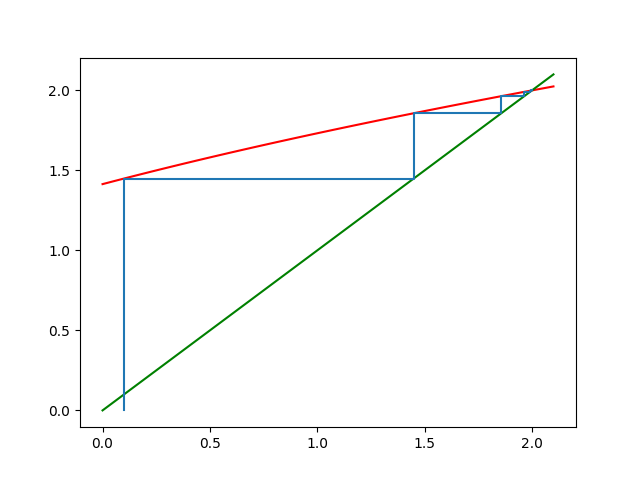
\includegraphics[scale=0.5]{suite.png} 
\end{center}
\item Refaire l'étude graphique de la suite $(u_k)_{k\in\mathbb{N}}$ dans les deux cas suivants:
\begin{itemize}
\item $\beta=0.7$ et $u_0=0.01$.
\item $\beta=0.82$ et $u_0=0.485$.
\end{itemize}
 \end{enumerate}

\subsection{Morpion}
Le morpion est un jeu de réflexion se pratiquant à deux joueurs (représentés par x et o) au tour par tour et dont le but est de créer le premier un alignement de trois de leurs symboles sur une grille.

 Le jeu peut se terminer par une égalité si l'ensemble le tableau se lève sans qu'aucun joueur ne termine une telle ligne. Vous devez écrire une simulation du jeu où un utilisateur (x) joue contre l'ordinateur (o). 


\begin{itemize}
\item nous pouvons supposer que l'utilisateur démarre toujours le jeu, en plaçant son marqueur x en premier sur le plateau.
\item si c'est au tour de l'utilisateur de jouer, il / elle entrera 2 entiers indiquant la  ligne et la colonne
de la cellule choisie. La cellule supérieure gauche est spécifiée par 0 0 et la cellule inférieure droite par 2 2. Votre programme doit assurer que la cellule sélectionnée est vide et demande à l'utilisateur de ressaisir une valeur au cas où la sélection choisie n'est pas possible.
\item si c'est au tour de l'ordinateur, une cellule parmi celles disponibles doit être choisie. Votre programme peut
utilisez n'importe quelle stratégie pour choisir la cellule. Par exemple, une sélection aléatoire parmi les cellules vides peut être choisi. Vous pouvez également utiliser une stratégie plus élaborée.
\end{itemize}





Votre programme doit stocker:
\begin{itemize}
\item  La liste des cellules vides restantes que l'on désigne par {\tt empty\_cells} sous forme de liste de couples (tuples) de coordonnées {\tt (row,col)}.
\item  L'état du jeu sous forme de liste de 3 listes, chacune représentant une ligne de la grille. par exemple la grille suivante: 

\begin{center}
\begin{tabular}{c|c|c|c|c}
&& & & \\ \hline
&o& &x & \\ \hline
&&o &o & \\ \hline
&x& &x & \\ \hline
&& & &  \\
\end{tabular}
\end{center}
est représentée par la variable:
\begin{verbatim}
g = [['o', '_', 'x'], ['_', 'o', 'o'], ['x', '_', 'x']]
\end{verbatim}
Les éléments  seront {\tt 'x'}, {\tt 'o'} ou {\tt '\_'} , désignant respectivement une cellule de l'utilisateur, une cellule de l'ordinateur ou une cellule vide.
\end{itemize}
L'affichage sera effectué par une fonction à double boucle for:
\begin{lstlisting}
# function d'affichage d'une liste de 3 listes
def print_grid(grid):
    for row in grid:
        for e in row:
            ...............
        print()
\end{lstlisting}

Voici quelques fonctions que vous voudrez peut-être écrire pour décomposer le programme en morceaux gérables.

\begin{itemize}
\item  {\tt getUserPick (empty\_cells, grid)} obtiendra le choix de l'utilisateur, s'assurera qu'il est valide et mettra à jour la grille.
\begin{lstlisting}
def get_user_pick(empty_cells, grid):
    global gUser
    while True:
        row = int(input("row= "))
        col = int(input("col= "))
        if (row,col) in empty_cells:
            grid[row][col]='x'
            empty_cells.remove((row,col))
            break
    print_grid(grid)
\end{lstlisting}

\item {\tt computerPick (empty\_cells, grid)} choisira une cellule parmi celles disponibles, mettra à jour la grille et supprimer la cellule choisie de la liste des cellules vides.
\begin{lstlisting}
def computer_pick(empty_cells, grid):
    while True:
        row = .........................
        col  = .........................
        if (row, col) in empty_cells:
            .........................
            .........................
            .........................
    .........................
\end{lstlisting}
\item {\tt checkWin (grille, joueur)} vérifie si le joueur (i.e., {\tt x}  ou {\tt o}) a gagné.
\begin{lstlisting}
def check_win(grid, player):
	# gridPlayer est la liste des coordonnées (row,col) des cases jouées par le joueur player (x ou o)
    gridPlayer = []
    for i in range(3):
        for j in range(3):
            .........................
                .........................
    #On teste s'il existe trois points alignés parmi les cases jouées par le player
    n=len(gridPlayer)
    for a in range(n):
        for b in range(a+1,n):
            for c in range(b+1,n):
                A = .....................
                B = .....................
                C = .....................
                # si det(vec(AB),vec(AC))=0 alors les trois points A,B et C sont alignés
                if .................................................. :
                    return True
    return False
\end{lstlisting}

\end{itemize}
Le programme principale ressemble à ceci:
\begin{lstlisting}
def tictactoe():
    empty_cells = []
    for i in range(3):
        for j in range(3):
            empty_cells.append((i, j))
    g = [['_', '_', '_'], ['_', '_', '_'], ['_', '_', '_']]
    while len(empty_cells)>0:
        print("-"*50)
        print("User : ")
        get_user_pick(empty_cells, g)
        if check_win(g, "x"):
            print("User wins !")
            return
        print("-"*50)
        print("Computer : ")
        computer_pick(empty_cells, g)
        if check_win(g, "o"):
            print("Computer wins !")
            return

# start the game
tictactoe()
\end{lstlisting}
Exemple d'exécution :
\begin{verbatim}
--------------------------------------------------
User : 
row= 1
col= 1
_ _ _ 
_ x _ 
_ _ _ 
--------------------------------------------------
Computer : 
_ o _ 
_ x _ 
_ _ _ 
--------------------------------------------------
User : 
row= 0
col= 0
x o _ 
_ x _ 
_ _ _ 
--------------------------------------------------
Computer : 
x o _ 
_ x _ 
o _ _ 
--------------------------------------------------
User : 
row= 2
col= 2
x o _ 
_ x _ 
o _ x 
User wins !
\end{verbatim}
\section{Récursivité}
\subsection{PGCD}
 Écrire une fonction récursive {\tt pgcd (a, b)} qui renvoie le plus grand commun diviseur de $a$ et $b$,  en utilisant le théorème d'Euclide $a\wedge b = b\wedge r$ où $r$ est le reste de la division euclidienne de $a$ par $b$. Lorsque $b = 0$, alors $a\wedge b =a$.
 \begin{lstlisting}
def pgcd(a,b):
    if b==0:
        return ......
    else:
        return .......

print(pgcd(102,68)) 
 \end{lstlisting}
\subsection{Inclusion}
Écrire une fonction récursive {\tt issubset (st1, st2)} qui prend deux arguments de chaînes de caractères et retourne {\tt True} si tous les caractères de la première chaîne {\tt st1} apparaissent quelque part dans {\tt st2}, et {\tt False} sinon.

Indication: 
\begin{itemize}
\item Si {\tt st1} est vide alors  {\tt issubset('', st2)=True}.
\item Si le premier caractère de st1  est dans st2 on a l'équivalence:

                      {\tt issubset(st1, st2)}$\Longleftrightarrow$ {\tt issubset(st1[1:], st2)}
\item Sinon {\tt issubset(st1, st2)=False}
\end{itemize}
\begin{lstlisting}
st1 = input("st1 = ")
st2 = input("st1 = ")

def issubset(st1,st2):
    if len(st1)==0:
        ............................
    else:
        if st1[0] in st2:
            ............................
        else:
           ............................


print(issubset(st1,st2))
\end{lstlisting}
\subsection{Palindrome en version récursive}
Écrire une fonction {\tt is\_palindrome2(st)},  version récursive d'une fonction déjà vu en TP1 qui renvoie un boolean indiquant  si son argument est ou non un palindrome.

Indication: 
\begin{itemize}
\item Si {\tt st} est vide ou contient un seul caractère alors  {\tt is\_palindrome2(st)=True}.
\item Si les deux caractères aux  extrémités de {\tt st}  sont égaux  alors on a l'équivalence:

                      {\tt is\_palindrome2(st)}$\Longleftrightarrow$ {\tt is\_palindrome2(st[1:-1])}
\item Sinon {\tt is\_palindrome2(st)=False}
\end{itemize}
\end{document}
\subsection{Fractales}
{\tt Turtle} est un module graphique de Python. Il permet de déplacer une tortue (souvent symbolisée par une flèche) sur l'écran d'une distance donnée {\tt forward(d)} selon une direction $+\alpha$ positive:  {\tt left($\alpha$)}  ou une direction $-\alpha$ négative:  {\tt right($\alpha$)} . Par exemple la fonction suivante permet de tracer un polygone régulier de $n$ côtés:
\begin{lstlisting}
from turtle import *
# polygone régulier de côté = 100 px
def polygone(n):
    for i in range(n):
      forward(100)
      left(360/n)

polygone(6)
\end{lstlisting}
Écrivez une fonction fractale récursive (ordre, longueur) qui trace une courbe fractale similaire à celles ci-dessous.

Une ligne fractale d'ordre 0 est un segment de droite d'une longueur donnée. Une ligne fractale d'ordre 1 est obtenue comme
suit: au lieu de dessiner une seule ligne, dessinez à la place quatre segments plus petits de longueur / 3 chacun et avec des angles de 60 ou 120 degrés. Une ligne fractale d'ordre 2 est obtenue en répétant le même motif sur chacun des segments d'ordre 1.

La répétition du motif nous donne à nouveau une ligne fractale d'ordre 3 telle que celle illustrée à droite ci-dessous.
\begin{center}
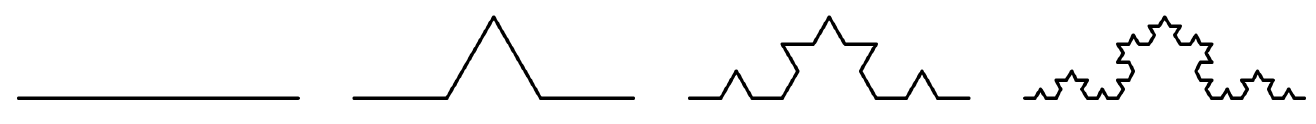
\includegraphics[scale=0.6]{fractale1.png} 
\end{center}
Écrire une fonction   {\tt snowflake(ordre, longueur)} qui dessine un fractal "snow
akes". Le flocon de neige  "snow akes" est un triangle équilatéral, où chaque côté est une ligne fractale d'un ordre et d'une longueur donnés.
\begin{center}
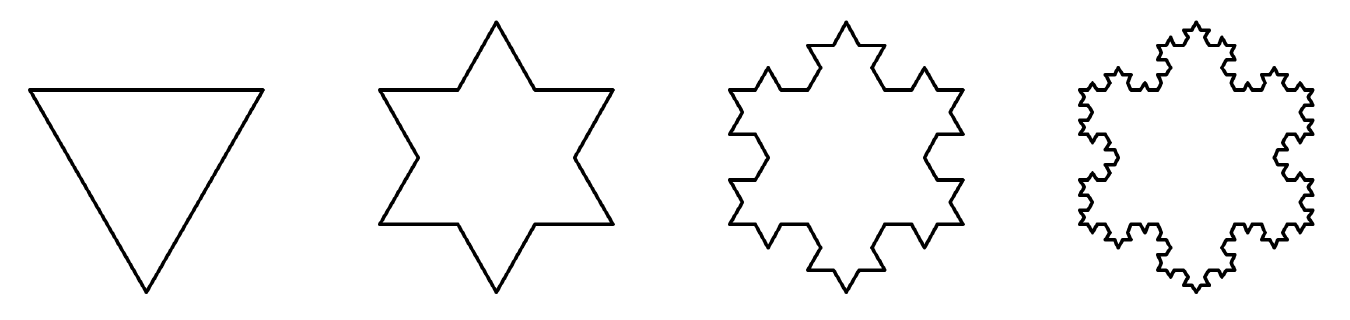
\includegraphics[scale=0.6]{fractale2.png} 
\end{center}
Remarque:  Le fractal "flocon de neige" est une forme qui a un certain nombre de propriétés curieuses: son  périmètre est infini tandis que son aire est finie (égale à 8/5 du triangle); sa limite est une courbe continue mais non dérivable en aucun points. 
\subsection{Arbres}
Écrivez une  fonction {\tt tree(n)} qui prend un argument entier $n$ et produit l'arbre récursif suivant. Exemples pour n = 1; 2; 3; 4; et 8 sont illustrés ci-dessous:
\begin{center}
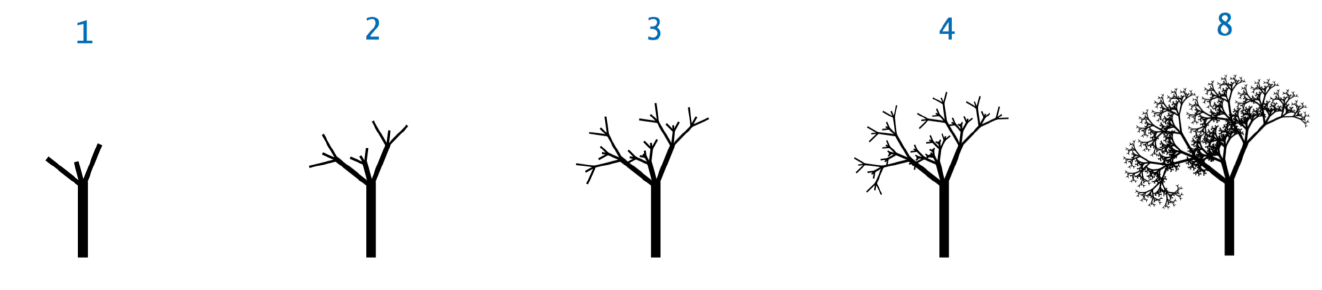
\includegraphics[scale=0.6]{fractale3.png} 
\end{center}
Pour cet exercice, il est demandé de tester et commenter uniquement, le code suivant:
\begin{lstlisting}
import turtle

def tree(n, length):
    if n>0:
        x = turtle.pos()
        widthFand=length / 15
        lenFand=0.618*length
        # 1
        turtle.right(23)
        turtle.width(widthFand)
        turtle.forward(lenFand)
        tree(n-1, lenFand)
        # 2
        turtle.goto(x)
        turtle.left(37)
        turtle.width(widthFand)
        turtle.forward(lenFand*0.4)
        tree(n - 1, lenFand)
        # 3
        turtle.goto(x)
        turtle.left(37)
        turtle.width(widthFand)
        turtle.forward(lenFand)
        tree(n - 1, lenFand)
        turtle.goto(x)
        turtle.right(51)

n = 4
turtle.left(90)
turtle.width(10)
turtle.forward(70)
tree(n, 70)
turtle.done()
\end{lstlisting}
\end{document}



















\subsection{Algèbre linéaire}

 \begin{enumerate}
\item On considère la matrice $A \in {\cal M}_{3,4}(\mathbb{R})$ définie par :
\[A=\left(\begin{array}{cccc}
4& 6 &-2& 3 \\
2 &-1& 0& 1 \\
-7& 0& 1 &12
\end{array}\right)\]
 \begin{enumerate}
\item Définir  la matrice $A$ comme un {\tt np.array()}. 
\item Modifier la matrice $A$ pour que ses deux premières lignes soient multipliées par 2 et que sa dernière colonne soit divisée par 3.
\item Créer une nouvelle matrice $B$ définie par
\[B=\left(\begin{array}{cccc}
4& 5 &6 \\
5 &10& 15 \\
1& 1& 1 
\end{array}\right)\]
en utilisant le fait que les lignes 1 et 2 sont composées des éléments successifs de deux suites arithmétiques (voir les fonctions {\tt np.arange} et {\tt np.ones()}).
\item Créer la matrice $C\in {\cal M}_{3,3}(\mathbb{R})$ extraite de $A$ telle que pour $1\leq i,j \leq 3$, $c_{ij} =a_{ij}$.
\item Calculer le produit matriciel $D$ de $B$ et $A$ ({\tt np.dot()}).
\item Calculer le produit d'Hadamard $E$ de $B$ et de $C$ défini par $\forall\; 1\leq i,j \leq 3$, $e_{ij} =b_{ij}\times c_{ij}$.
\item Calculer la somme des éléments de la matrice $E$ et le vecteur colonne $Y\in \mathbb{R}^3$ tel que pour $1\leq i\leq 3$, $y_i=\sum_{i=1}^3d_{ij}$. ({\tt np.sum()})

\end{enumerate}
\item On considère la matrice $A \in {\cal M}_{4}(\mathbb{R})$ suivante
\[A=\left(\begin{array}{cccc}
4& 5 &6& -1\\
5 &10& 15& 2 \\
6& 15& 1 &4\\
-1&2&4&-2
\end{array}\right)\]

\begin{enumerate}
\item Montrer, à l'aide de Python, que $A$ est diagonalisable.
\item  Calculer ses valeurs propres et donner une base de vecteurs propres ({\tt np.linalg.eig()}).
\item  Calculer de deux manières l'inverse de $A$ en utilisant le résultat précédent et la fonction {\tt np.linalg.inv}. Comparer les résultats obtenus (vous pourrez regarder la librairie {\tt matplotlib} pour faire des tracés avec Python)
\end{enumerate}
\item On considère maintenant la matrice $A \in {\cal M}_{n}(\mathbb{R})$: 
\[A=\left(\begin{array}{cccccc}
2& -1 &0& \cdots &\cdots & 0\\
-1 &2& -1 & \ddots& \ddots&\vdots  \\
0 & \ddots& \ddots& \ddots& \ddots& \vdots  \\
\vdots & \ddots& \ddots& \ddots& \ddots& 0 \\
\vdots & \ddots& \ddots& -1& 2& -1 \\
0 & \cdots&\cdots& 0& -1& 2
\end{array}\right)\]
Examiner, comme à la question précédente, les cas $n = 5, 10, 50$ (on utilisera $n$ comme une variable, et on devra construire la matrice avec {\tt np.eyes()} en fonction de $n$). Comparer les valeurs propres obtenues avec les valeurs définies pour $1\leq k\leq n$ par
\[\lambda_k=4\sin^2\left(\frac{k\pi}{2(n+1)}\right)\]
(On pourra utiliser la fonction {\tt np.sort()})
\item On s'intéresse à la matrice $M \in {\cal M}_{3,5}(\mathbb{R})$:
\[M=\left(\begin{array}{ccccc}
1& -1 &2&1 &2\\
-1 &2& 3 & -4& 1  \\
0 & -1& 1& 0&0  
\end{array}\right)\]
\begin{enumerate}
\item Quel est le rang de la matrice $M$? Utiliser la fonction {\tt np.linalg.matrix\_rank} afin de retrouver ce résultat.
\item En définissant:
\[A=\left(\begin{array}{ccccc}
1& -1 &2\\
-1 &2& 3  \\
0 & -1& 1
\end{array}\right), \mbox{ et } b=\left(\begin{array}{c}
3\\
-7  \\
 1
\end{array}\right)  \]
résoudre à l'aide de la fonction {\tt np.linalg.solve()} le système $Ax = b$.
\end{enumerate}
\end{enumerate}
\subsection{Tableaux bidimensionnels et découpage}
 \noindent Créez un tableau $4\times 4$ avec des valeurs arbitraires, puis
 \begin{enumerate}
\item Extraire les éléments de la deuxième ligne.
\item  Extraire les éléments de la troisième colonne.
\item  Attribuez une valeur de 3 à la sous-matrice $2\times 2$ supérieure gauche.
 \end{enumerate}

\subsection{Division et combinaison de tableaux }
\noindent Continuer avec le tableau $4\times 4$ précédent:

\begin{enumerate}
\item Utilisez la fonction {\tt np.split()} pour diviser le tableau en deux nouveaux tableaux $2\times 4$.
Reconstruisez le tableau $4\times 4$ d'origine en utilisant {\tt np.concatenate()}.
\item Répétez l'exercice ci-dessus, mais créez maintenant des sous-tableaux $4\times 2$, puis combinez-les.
\end{enumerate}
\begin{itemize}
\item[$\bullet$] {\tt np.split(ary,indices\_ou\_sections, axis=0)}
\begin{itemize}
\item {\tt ary}: le tableau ndarray à diviser en sous-tableaux
\item {\tt indices\_ou\_sections} est un nombre entier, $N$, le tableau sera divisé en $N$ tableaux égaux le long de l’axe. Si une telle division n'est pas possible, une erreur est générée.
 Si {\tt  indices\_ou\_sections} est un tableau 1D d'entiers triés, les entrées indiquent où, le long de l'axe, le tableau est divisé.
\item Axis: int, facultatif, 0 par défaut
\end{itemize}
\item[$\bullet$] {\tt np.concatenate((ary1,ary2),axis,out=None)}
\begin{itemize}
\item {\tt ary1, ary2}: les tableaux doivent avoir la même forme, sauf dans la dimension correspondant à l'axe
\item {\tt axis}: int, facultatif, l'axe le long duquel les tableaux seront joints
\item {\tt out}: la destination pour placer le résultat.
\end{itemize}

\end{itemize}

\section{Analyse numérique}
\subsection{Différenciation numérique}
On définit la fonction $f$ sur l'intervalle $[-2\pi,2\pi]$ par $f(x)=\frac 12\cos(2x)-cos(x)$. 
\begin{enumerate}
\item Tracer $f$ et sa dérivée $f'$ en choisissant une discrétisation de $[-2\pi,2\pi]$ en $N=100$ points.
\item  La dérivée de $f$ peut être calculée numériquement par une méthode des différences finies comme suit:
\[f'(x_i)=\frac{f(x_i+\Delta x)-f(x_i-\Delta x)}{2\Delta x}
\]
Écrire une fonction {\tt df} permettant de calculer un tableau 1D Numpy contenant les dérivées approchées de $f$ aux points $x_i$ d'une discrétisation de l'intervalle $[-2\pi,2\pi]$ en $n=30$. Essayez d'éviter les boucles. Comparez le résultat à la fonction $f'$ dans le même intervalle.
\end{enumerate}

\subsection{Polynômes}
Approcher un polynôme du second degré aux données de l'exercice précédent en utilisant {\tt numpy.polyfit()}. Tracer le graphique représentant toutes les données.
%\subsection{Algèbre linéaire}
%Construire deux matrices $2\times 2$ symétriques $A$ et $B$.
%(indice: une matrice symétrique peut être construite facilement comme $A_{sym} = A + A^t$)
%Calculez le produit de la matrice $C = A * B$ en utilisant {\tt numpy.dot()}.
%Calculez les valeurs propres de la matrice $C$ avec {\tt numpy.linalg.eigvals()}.
\subsection{Graphique simple}
Tracez sur le même graphe les fonctions $\sin$ et $\cos$ dans l'intervalle $[-\pi / 2, -\pi / 2]$. Utilisez $\theta$ comme $x-$label et insérez aussi les légendes. Enregistrez la figure au format {\tt .png} .
Tracez les mêmes fonctions sur deux graphiques séparés en utilisant 2 méthodes.
\subsection{Intégration}
 Le module d’intégration {\tt scipy.integrate} contient des outils d’intégration numérique. Utilisez le module pour évaluer les intégrales
 \[\int_1^{3.5}(1+x^2){\mbox d}x \quad {\mbox et}\quad \int_0^\infty \exp(-x^2) {\mbox d}x \]
 \subsection{Optimisation}
 Trouver, s'il existe, le minimum de la fonction réelle définie par
 \[ f(x)=(x+4)(x+1)(x-1)(x-3)\]
en utilisant la fonction {\tt minimize\_scalar()} du module {\tt scipy.optimize}.
\subsection{Série de Riemann}
Une méthode simple pour évaluer numériquement les intégrales est la somme de Riemann du milieu

\[ S=\sum_{i=1}^nf(x'_i)\Delta x \]

où $x’_i = \frac{x_i + x_{i-1}}2$. Utilisez le même intervalle que dans le premier exercice et déterminez dans quelle mesure la somme de Riemann diffère de $0.1$ de la valeur de l'intégrale correspondant. Évitez les boucles. Recherchez également comment les résultats changent avec le choix de $\Delta x$.
%\section{Mécanique du point: Pendule simple à ressort}
%%  06 7779 3344  René
%Comme vous vous en doutez, {\tt Scipy} a une routine \href{https://docs.scipy.org/doc/scipy/reference/generated/scipy.integrate.odeint.html} {\tt odeint()}  qui résout les équations différentielles. Cette fonction est disponible sous {\tt scipy.integrate.odeint()}. Elle utilise des tailles de pas variables et des méthodes de vérification des erreurs pour obtenir des résultats très précis, de manière efficace. Appelez cette routine avec une fonction dérivative, une valeur d'état initiale (qui peut-être un tableau, comme d'habitude) et un tableau de fois (plutôt qu'un pas de temps). La fonction {\tt scipy.integrate.odeint()} retournera un tableau de valeurs d'état en fonction du temps. 
%
% \begin{wrapfigure}{r}{0.25\textwidth} %this figure will be at the right
%    \centering
%% \includegraphics[scale=0.3]{pendule.png} 
% \includegraphics[width=0.25\textwidth]{pendule.png}
%\end{wrapfigure}
% Une masse $m$ est attachée à un ressort de raideur $k$, qui est attachée à un point de support, comme indiqué dans la figure ci-dessous. La longueur du pendule résultant à un instant donné est égale à la longueur de repos du ressort $\ell_0$ plus l'allongement (ou la compression) $\ell$, et l'angle du pendule par rapport à la verticale est égal à $\theta$. Voici un exemple de système oscillateur couplé: les oscillations «pendulaires» d'écart $\theta$ interagissent avec les oscillations «de ressort» d'allongement $\ell$, produisant un mélange complexe des deux. Les équations différentielles pour ce système sont données par
% \[ \ell''=(\ell_0+\ell)\theta'^2-\frac{k}{m}\ell+g\cos\theta \]
%  \[ \theta''=-\frac 1{\ell_0+\ell}\left(2\ell' \theta'+g\sin\theta\right) \]
%  
%  Écrivez un programme qui trace le mouvement de la masse pour une $\theta \neq 0$  initiale.
%
%Suivez ces étapes :
%
%\begin{enumerate}
%\item Définissez d'abord les variables initiales et placez-les dans un tableau de dimension $= 1$ et {\tt shape = (4,)}.\\
%Nous avons en fait quatre paramètres à suivre (position et vitesse):
%    \[\ell ,\quad \ell',\quad \theta \quad{\mbox et }\quad \theta’\]
%Les valeurs initiales sont $\ell_0=1$, $\ell=0$ , $\ell'=0$, $\theta=0.3$  et  $\theta’=0$.
%
%\item Définir les pas de temps. Pour résoudre ce problème, nous devons itérer dans le temps. Pour chaque instant $t$, nous mettrons à jour les valeurs des quatre paramètres.
%Prenons par exemple $N = 1000$ (nombre de pas de temps).
%Définissez un tableau de pas de temps pour faire $1000$ itérations. La fin de la simulation devrait être à $t = 25 s$
%
%\item Définissez une fonction qui prendra le tableau des quatre paramètres (1.) et le tableau du temps (2.). Cette fonction devrait calculer les dérivées des paramètres et les renvoyer.
%
%\item Définissez un tableau $N\times 4$ en utilisant simplement la fonction {\tt scipy.integrate.odeint()}.
%
%\item Enfin, tracez les données.
%\end{enumerate}
%%%%%%%%%%%%%%%%%%%%%%%%%%%%%%%%%%%%%%%%%%%%%%%%%%%%%%%%%%%%%%%%%%%%%%%%%%%%%%%


\end{document}


